\documentclass{ximera}

\title{Theory}
\author{Mila Vervoort}
\license{CC: 0}         % replace with an appropriate license, or set it in xmPreamble

\begin{document}
\begin{abstract}
    Samenvatting van de theorie over ideale homogene reactoren onder isotherme voorwaarden.
\end{abstract}
\maketitle
\label{xim:theory}

In hoofdstuk 3 'Ontwerp van homogene reaktoren onder isotherme werkingsvoorwaarden' werd gezien hoe door het opstellen van de stofbalans de nodige ontwerpvergelijkingen bekomen kunnen worden. 

\begin{definition} 
Stofbalans\\
Een stofbalans is van de volgende vorm: 
\[
\text{Accumulatie} = \text{In} - \text{Uit} + \text{Reactie} 
\]
In formulevorm:
\[
\frac{dN_A}{dt} = F_{A,in} - F_{A,out} + R_A V
\]
waar:
\begin{itemize}
\item $N_A$ = aantal mol van component A in de reactor
\item $F_{A,in}$ = molstroom van A naar binnen
\item $F_{A,out}$ = molstroom van A naar buiten
\item $R_A$ = reactiesnelheid van A (mol/(m$^3$s))
\item $V$ = reactorvolume
\end{itemize}
\end{definition}

\begin{remark}
Monotoon stijgende kinetica

We veronderstellen een monotoom stijgende kinetiek in het vervolg van de theorie.
Voor een irreversibele reactie met monotoon stijgende kinetica geldt:

\[
R_A = \frac{dC_A}{dt} = -k C_A^n
\]

waarbij:

\begin{itemize}
\item $n=1$ : eerste orde
\item $n=2$ : tweede orde
\item $n=3$ : derde orde
\item $\dots$
\end{itemize}

Verder volgt dat:

\[
-\frac{1}{R_A} = \frac{1}{k C_A^n}
\]

De onderstaande grafiek toont $-1/R_A$ als functie van $C_A$
voor verschillende waarden van de reactie-orde $n$. 

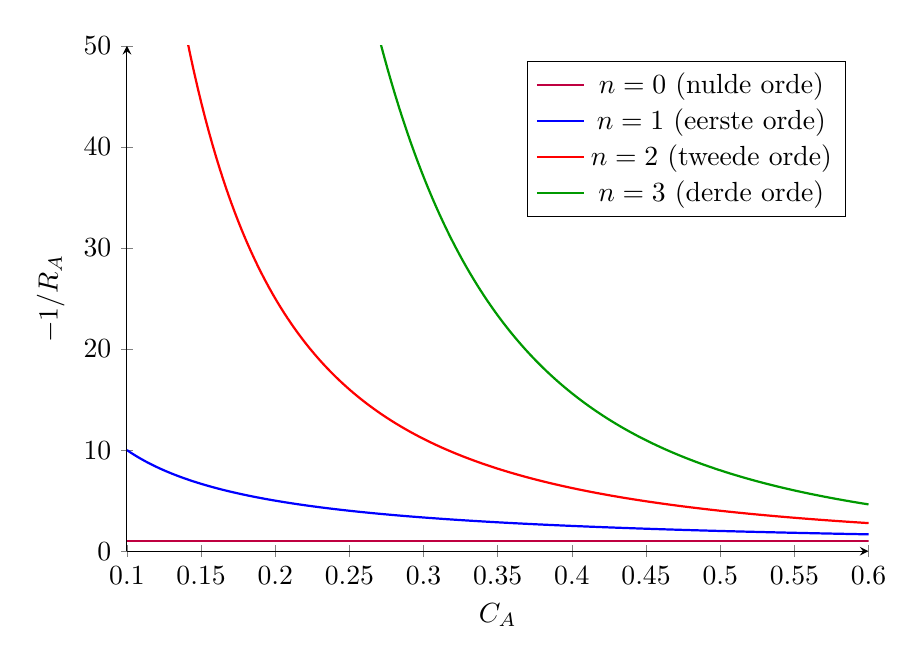
\begin{tikzpicture}
\begin{axis}[
    xlabel={$C_A$},
    ylabel={$-1/R_A$},
    domain=0.1:0.6,
    samples=200,
    axis lines=left,
    width=11cm,
    height=8cm,
    legend pos=north east,
    ymin=0,
    ymax=50,
]
% n = 0
\addplot[purple, thick] {1};
\addlegendentry{$n=0$ (nulde orde)}

% n = 1
\addplot[blue, thick] {1/x};
\addlegendentry{$n=1$ (eerste orde)}

% n = 2
\addplot[red, thick] {1/(x^2)};
\addlegendentry{$n=2$ (tweede orde)}

% n = 3
\addplot[green!60!black, thick] {1/(x^3)};
\addlegendentry{$n=3$ (derde orde)}

\end{axis}
\end{tikzpicture}
\end{remark}

\begin{remark}
\textbf{Variabele densiteit}

In veel reacties is de densiteit van het reagerend mengsel niet constant. 
Wanneer tijdens de reactie het aantal mol gas toeneemt of afneemt, zal ook het totale volume veranderen. 
Het controlevolume wordt dus een functie van de reactievoortgang.

Als lineaire benadering wordt aangenomen:
\[
V = V_0 (1 + \varepsilon_A X_A)
\]
Hierbij is:
\begin{itemize}
    \item $V_0$ het beginvolume,
    \item $X_A$ de conversie van component $A$,
    \item $\varepsilon_A$ de expansiefactor.
\end{itemize}

De expansiefactor $\varepsilon_A$ geeft weer hoe sterk het volume verandert bij volledige omzetting van $A$:
\[
\varepsilon_A = \frac{V_{X_A=1} - V_0}{V_0}
\]

Hieruit volgt:
\begin{itemize}
    \item $\varepsilon_A > 0$ : expansie (toename van het volume),
    \item $\varepsilon_A < 0$ : compressie (afname van het volume).
\end{itemize}
\end{remark}


 
\section{Batch Reactor}

In een batch reactor is er geen in- of uitstroom (\(F_{A,in} = F_{A,out} = 0\)):

\[
\frac{dN_A}{dt} = R_A V
\]

Aangezien $N_A = N_{A0}(1-X_A)$:

\[
\frac{dX_A}{dt} = \frac{-r_A}{C_{A0}}
\]

Om de tijd \(t\) te berekenen die nodig is om van een initiële conversie \(X_{A0} = 0\) naar conversie \(X_A\) te gaan, integreren we:

\[
\boxed{
t = \int_0^{X_A} \frac{C_{A0}}{-r_A}\, dX_A
}
\]

\begin{image}
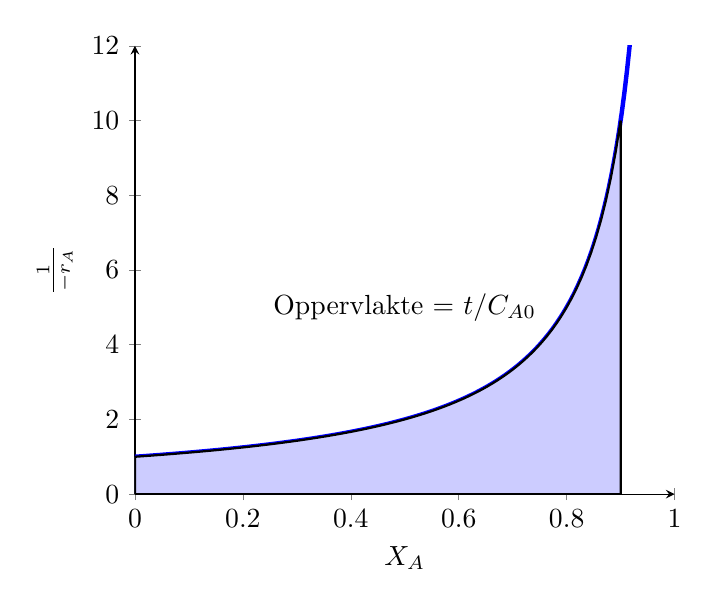
\begin{tikzpicture}
\begin{axis}[
    domain=0:0.95,
    samples=200,
    xmin=0, xmax=1,
    ymin=0, ymax=12,
    axis lines=left,
    xlabel={$X_A$},
    ylabel={$\frac{1}{-r_A}$},
]

% parameters
\addplot[ultra thick, blue]
{1/(1*(1-x))};

% arceer het gebied tussen C_A_end en C_A0
\addplot [
    thick,
    fill=blue!20,
    domain=0:0.9,   % van C_A,e tot C_A0
    samples=100
] {1/(1*(1-x))} \closedcycle;

% Voeg een t label toe in het gearceerde gebied
\node at (axis cs:0.5,5) {Oppervlakte = $t/C_{A0}$};

\end{axis}
\end{tikzpicture}
\end{image} 

Bij de aanname van constante densiteit en dus een constant controlevolume, kan de molaire hoeveelheid omgevormd worden naar de concentratie van reagens A.

\[
\frac{dC_A}{dt} = r_A
\]

Om de tijd \(t\) te berekenen die nodig is om van een initiële concentratie \(C_{A0}\) naar \(C_A\) te gaan, integreren we:
\[
\boxed{
t = \int_{C_{A0}}^{C_A} \frac{dC_A}{r_A}
}
\]

\begin{image}
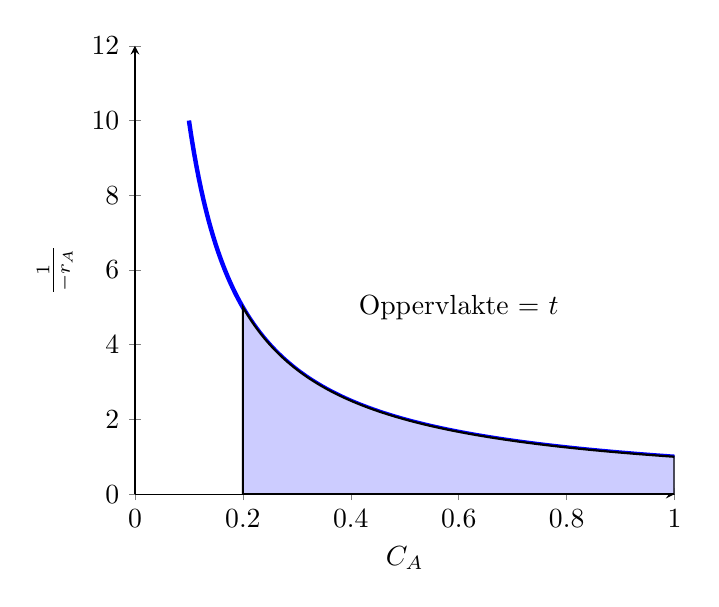
\begin{tikzpicture}
\begin{axis}[
    domain=0.1:1,       % x loopt van 0 tot C_A0
    samples=200,
    xmin=0, xmax=1,
    ymin=0, ymax=12,
    axis lines=left,
    xlabel={$C_A$},
    ylabel={$\frac{1}{-r_A}$},
]

% parameters
\def\k{1}   % snelheidsconstante

% plot de curve
\addplot[ultra thick, blue] {1/(\k*x)};

% arceer het gebied tussen C_A_end en C_A0
\addplot [
    thick,
    fill=blue!20,
    domain=0.2:1,   % van C_A,e tot C_A0
    samples=100
] {1/(\k*x)} \closedcycle;

% Voeg een t label toe in het gearceerde gebied
\node at (axis cs:0.6,5) {Oppervlakte = $t$};

\end{axis}
\end{tikzpicture}
\end{image}


\section{CSTR (Continuous Stirred Tank Reactor)}

In een CSTR met constante in- en uitstroom geldt bij stationaire toestand:

\[
0 = F_{A0}-F_A+r_A V
\]

\[
F_{A0}X_A = -r_A V
\]

\[
\boxed{
\frac{V}{F_{A0}} = \frac{X_{Ae}}{-r_A(X_{Ae}}
}
\]

\begin{image}
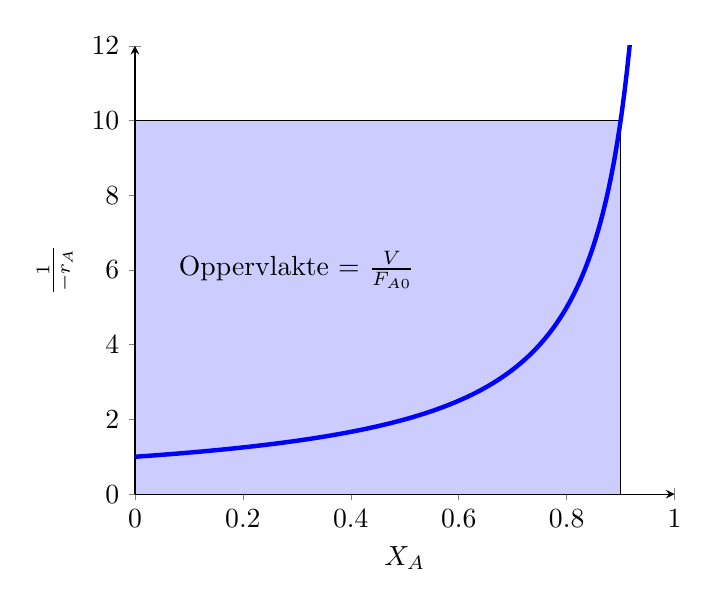
\begin{tikzpicture}
\begin{axis}[
    domain=0:0.95,
    samples=200,
    xmin=0, xmax=1,
    ymin=0, ymax=12,
    axis lines=left,
    xlabel={$X_A$},
    ylabel={$\frac{1}{-r_A}$},
]


% arceer het gebied 
\draw[fill=blue!20] 
    (axis cs:0,0) rectangle 
    (axis cs:0.9,{1/(1-0.9)});

% parameters
\addplot[ultra thick, blue]
{1/(1*(1-x))};

\node at (axis cs:0.3,6) {Oppervlakte = $\frac{V}{F_{A0}}$};


\end{axis}
\end{tikzpicture}
\end{image} 

Bij de aanname van constante densiteit:

\[
\boxed{
\tau = \frac{C_{A0}-C_{Ae}}{-r_A(C_{Ae})}
}
\]


\begin{image}
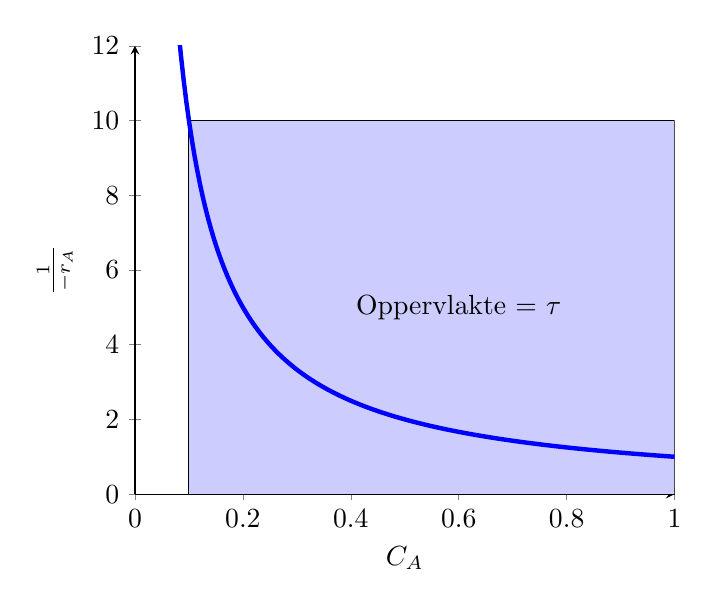
\begin{tikzpicture}
\begin{axis}[
    domain=0:1,       % x loopt van 0 tot C_A0
    samples=200,
    xmin=0, xmax=1,
    ymin=0, ymax=12,
    axis lines=left,
    xlabel={$C_A$},
    ylabel={$\frac{1}{-r_A}$},
]

% parameters
\def\k{1}   % snelheidsconstante



% arceer het gebied 

\draw[fill=blue!20] 
    (axis cs:1,0) rectangle 
    (axis cs:0.1,{1/0.1});
% plot de curve
\addplot[ultra thick, blue] {1/(\k*x)};
    
% Voeg een t label toe in het gearceerde gebied
\node at (axis cs:0.6,5) {Oppervlakte = $\tau$};

\end{axis}
\end{tikzpicture}
\end{image}


\section{PFR (Plug Flow Reactor)}

In een PFR verandert de concentratie langs de reactorlengte \(x\). De stofbalans over een klein segment \(dV\) is:


\[
\frac{dF_A}{dV} = r_A
\]

\[
\frac{dX_A}{dV} = \frac{-r_A}{F_{A0}}
\]

\[
\boxed{
\frac{V}{F_{A0}} = \int_0^{X_{Ae}}\frac{dX_A}{-r_A}
}
\]


\begin{image}
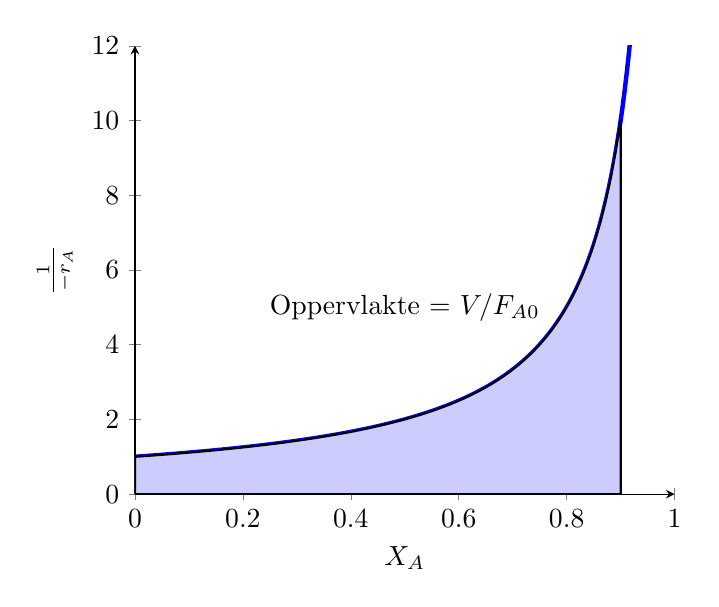
\begin{tikzpicture}
\begin{axis}[
    domain=0:0.95,
    samples=200,
    xmin=0, xmax=1,
    ymin=0, ymax=12,
    axis lines=left,
    xlabel={$X_A$},
    ylabel={$\frac{1}{-r_A}$},
]

% parameters
\addplot[ultra thick, blue]
{1/(1*(1-x))};

% arceer het gebied tussen C_A_end en C_A0
\addplot [
    thick,
    fill=blue!20,
    domain=0:0.9,   % van C_A,e tot C_A0
    samples=100
] {1/(1*(1-x))} \closedcycle;

% Voeg een t label toe in het gearceerde gebied
\node at (axis cs:0.5,5) {Oppervlakte = $V/F_{A0}$};

\end{axis}
\end{tikzpicture}
\end{image} 

Bij de aanname van constante densiteit:

\[
\boxed{
\tau = - \int_{C_{A0}}^{C_{Ae}} \frac{dC_A}{-r_A}
}
\]

\begin{image}
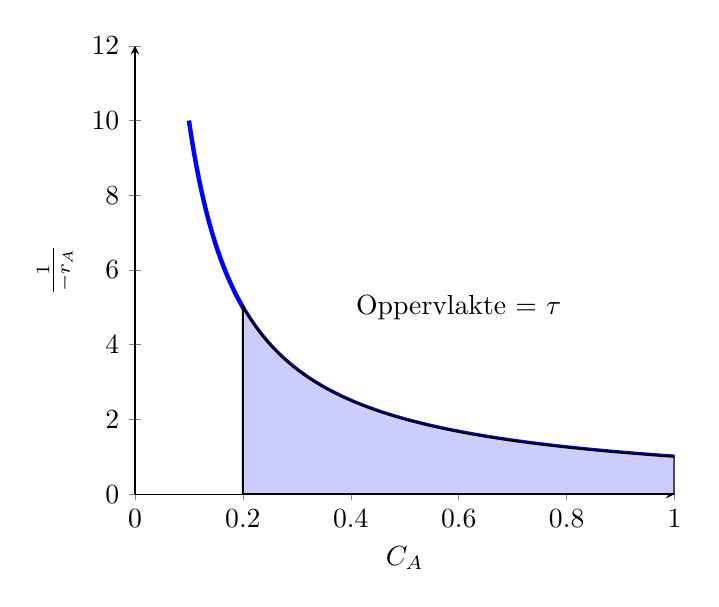
\begin{tikzpicture}
\begin{axis}[
    domain=0.1:1,       % x loopt van 0 tot C_A0
    samples=200,
    xmin=0, xmax=1,
    ymin=0, ymax=12,
    axis lines=left,
    xlabel={$C_A$},
    ylabel={$\frac{1}{-r_A}$},
]

% parameters
\def\k{1}   % snelheidsconstante

% plot de curve
\addplot[ultra thick, blue] {1/(\k*x)};

% arceer het gebied tussen C_A_end en C_A0
\addplot [
    thick,
    fill=blue!20,
    domain=0.2:1,   % van C_A,e tot C_A0
    samples=100
] {1/(\k*x)} \closedcycle;

% Voeg een t label toe in het gearceerde gebied
\node at (axis cs:0.6,5) {Oppervlakte = $\tau$};

\end{axis}
\end{tikzpicture}
\end{image}

\section{Vergelijking van ideale reactoren}
\subsection{Vergelijking: CSTR vs PFR}

We vergelijken de verblijftijd voor eenzelfde uitgangsconcentratie $C_A$.

\[
\tau_{PFR} = \int_{C_{A0}}^{C_{Ae}} \frac{dC_A}{r_A}
\]

\[
\tau_{CSTR} = \frac{C_{A0}-C_{Ae}}{-r_A(C_{Ae})}
\]

Grafisch in een $-1/r_A$ versus $C_A$ diagram:

\begin{center}
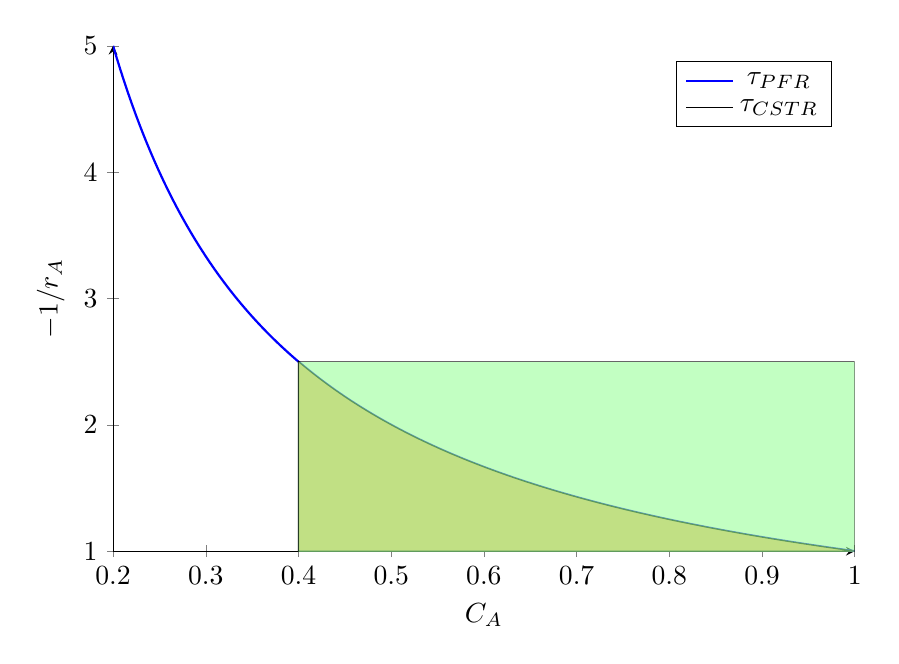
\begin{tikzpicture}
\begin{axis}[
    xlabel={$C_A$},
    ylabel={$-1/r_A$},
    domain=0.2:1,
    samples=200,
    axis lines=left,
    width=11cm,
    height=8cm,
    legend pos=north east,
]

% kinetiek
\addplot[blue, thick] {1/x};

% PFR oppervlakte
\addplot[
    domain=0.4:1,
    fill=orange!60
] {1/x} \closedcycle;
\addlegendentry{$\tau_{PFR}$}

% CSTR rechthoek
\draw[fill=green!40, opacity=0.6]
    (axis cs:1,0)
    rectangle
    (axis cs:0.4,{1/0.4});
\addlegendentry{$\tau_{CSTR}$}

\end{axis}
\end{tikzpicture}
\end{center}

\textbf{Interpretatie:}

Bij monotoon stijgende kinetica:


\[
\tau_{CSTR} > \tau_{PFR}
\]

Een PFR is dus meer performant dan een CSTR voor dezelfde conversie.

Dit kan je ook zelf even uittesten:
\begin{center}
\geogebra{m4v7cs3y}{700}{500}
\end{center}

\subsection{Vergelijking: Batch vs PFR}

Voor constante densiteit hebben Batch en PFR dezelfde
integraalvorm.

\begin{center}
\begin{tikzpicture}
\begin{axis}[
    xlabel={$C_A$},
    ylabel={$-1/r_A$},
    domain=0.2:1,
    samples=200,
    axis lines=left,
    width=11cm,
    height=8cm,
    legend pos=north east,
]

% kinetiek
\addplot[blue, thick] {1/x};
\addlegendentry{$-1/r_A$}

% PFR oppervlakte
\addplot[
    domain=0.4:1,
    fill=orange!40
] {1/x} \closedcycle;
\addlegendentry{$\tau_{PFR}$}

% Batch oppervlakte (zelfde gebied, andere kleur rand)
\addplot[
    domain=0.4:1,
    draw=red,
    pattern=north east lines,
    pattern color=red
] {1/x} \closedcycle;
\addlegendentry{$t_{Batch}$}

\end{axis}
\end{tikzpicture}
\end{center}

\textbf{Interpretatie:}

Bij constante densiteit is:

\[
t_{Batch} = \tau_{PFR}
\]

De tijd dat een fluidumelement verblijft in een propstroom reactor en in een batch reactor zijn equivalent.

\section{PFR met recyclestroom}
We beschouwen een plug flow reactor (PFR) met een externe recyclestroom.
De verse voeding heeft volumestroom $q$ en concentratie $C_{A0}$.
Een deel van de uitstroom wordt teruggevoerd naar de ingang van de reactor.

\begin{image}
\includegraphics[width=5cm]{PFR_met_recycle.png}
\end{image} 

\begin{itemize}
\item $q$ = volumestroom van de verse voeding
\item $R$ = recycleverhouding (dimensionloos)
\item Recycledebiet = $R q$
\item Totaal debiet door de reactor = $q (R+1)$
\item $C_{A,in}$ = concentratie aan de reactorinlaat
\item $C_{A,uit}$ = concentratie aan de reactoruitlaat
\item $V$ = reactorvolume
\end{itemize}

We nemen aan:
\begin{itemize}
\item constante dichtheid
\item stationaire toestand
\end{itemize}

De verse stroom en de recyclestroom mengen perfect vóór de reactor.
Daaruit volgt:
\[
q C_{A0} + R q C_{A,uit} = q (R+1) C_{A,in}
\]
Hieruit volgt:
\[
C_{A,in} = \frac{C_{A0} + R C_{A,uit}}{R+1}
\]
De inlaatconcentratie ligt dus tussen $C_{A0}$ en $C_{A,uit}$.\\

Vervolgens kunnen we voor deze reactor ook de stofbalans opstellen. 
\[
\text{Accumulation} = \text{In} - \text{Uit} + \text{Vorming} - \text{Verbruik}
\]
Voor een differentieel volume-element $dV$ geldt bij stationaire toestand:
\[
q(R+1)C_A - q(R+1)(C_A + dC_A) + r_A dV = 0
\]

Vereenvoudigen geeft:
\[
q(R+1)\, dC_A = r_A \, dV
\]
of
\[
\frac{dV}{q} = (R+1)\frac{dC_A}{-r_A}
\]
Integreren van $C_{A,in}$ tot $C_{A,uit}$ levert:
\[
\tau = \frac{V}{q} 
= (R+1)\int_{C_{A,uit}}^{C_{A,in}} \frac{dC_A}{-r_A}
\]

\begin{remark}
Fysische interpretatie 

De recycleverhouding R kan variëren van $0$ tot $\infty$
\begin{itemize}
\item Als $R = 0$:
\[
C_{A,in} = C_{A0}
\]
Het systeem reduceert tot een gewone PFR.
\item Als $R \rightarrow \infty$:
\[
C_{A,in} \rightarrow C_{A,uit}
\]
Er treedt sterke menging op en het gedrag benadert dat van een CSTR.
\end{itemize}
\end{remark}

\subsection*{Effect van recycle}
Voor een isotherm proces met monotoon stijgende kinetiek geldt dat de reactiesnelheid afneemt met dalende concentratie. In dat geval is een ideale PFR ($R=0$) het meest volume-efficiënt.\\

Het toevoegen van recycle verhoogt het totale debiet door de reactor met een factor $(R+1)$ en verlaagt de inlaatconcentratie. Hierdoor wordt de gemiddelde reactiesnelheid kleiner en neemt het benodigde volume om dezelfde conversie te behalen toe. In de limiet $R \rightarrow \infty$ wordt het vereiste volume gelijk aan dat van een CSTR.\\

\begin{image}
\includegraphics[width=5cm]{Volume_recycle.png}
\end{image} 

Recycle is dus voor zuiver isotherme systemen met eenvoudige, 
monotoon stijgende kinetiek niet gunstig vanuit volume-oogpunt. 
Bij niet-isotherme processen of complexere kinetiek kan recycle 
echter wél voordelig zijn.



\end{document}